\section{Evaluation}
\subsection{Prüfung der Anforderungen}

Dieser Abschnitt behandelt in wieweit das beschriebene Konzept die in Abschnitt \ref{anforderungen} aufgelisteten Anforderungen erfüllt. Die jeweilige Anforderung wird zunächst wiederholt und anschließend genauer untersucht.

\subsubsection{1) Transparente Einzahlungen}
\textit{Die Einzahlung jedes Endnutzers ist für jeden anderen Endnutzer nachprüfbar.}\\\\
Einzahlungen geschehen genau wie bei Bitcoin innerhalb von Transaktionen, die in die Blockchain geschrieben werden. Diese Anforderung ist also auch im Falle von Ethereum erfüllt.
\subsubsection{2) Gewinnerauswahl durch Zufallsfaktor}
\textit{Die Auswahl des Gewinners ist von einem zufälligen Faktor abhängig, auf den weder die Anwendung noch die Endnutzer einen Einfluss haben.}\\\\
Genau wie bei Bitcoin findet die Gewinnerauswahl basierend auf einem aus dem Proof-of-Work Blockhash statt. Die in Abschnitt \ref{btc_evaluation} betrachtete Analyse gilt somit genauso für Ethereum außer, dass der Mining Reward 3 Ether beträgt und durchschnittlich alle 12 Sekunden ausgeschüttet wird. In Zukunft plant Ethereum von einem Proof-of-Work Algorithmus auf einen Proof-of-Stake Algorithmus umzusteigen. Proof-of-Stake und die daraus resultierenden Auswirkungen werden in Kapitel \ref{pos} betrachtet.
\subsubsection{3) Nachprüfbarkeit des Zufallsfaktors}
\textit{Jeder Endnutzer kann die Echtheit des zufälligen Faktors eigenständig nachprüfen.}\\\\
Der zur Gewinnerauswahl verwendete Blockhash ist zum Zeitpunkt der Auszahlung bereits in der öffentlichen Blockchain verankert und kann somit überprüft werden.
\subsubsection{4) Transparente Auszahlungen}
\textit{Die Auszahlung an den Gewinner muss transparent und somit für jeden Endnutzer nachprüfbar sein.}\\\\
Die Auszahlung wird durch die vom Nutzer initiierte \code{payout} Transaktion ausgelöst und vom Smart Contract vorgenommen. Das Verfahren der Auszahlung ist durch den unveränderlichen Smart Contract Code in Stein gemeißelt. Die Konsensregeln und die dahinter liegende Spieltheorie garantieren, dass dieser auch genauso ausgeführt wird. Obwohl die \code{payout} Transaktion nicht direkt Geld auf die Auszahlungsadresse des Gewinners überweist, kann der Endnutzer dennoch sicher sein, dass eine Auszahlung stattgefunden hat, wenn die \code{payout} Transaktion wie in Abbildung \ref{fig:contract_payout_txn} im Status \code{success} vorliegt.
\subsubsection{5) Fairheit des Spiels}
\textit{Jeder Endnutzer besitzt die gleiche Gewinnwahrscheinlichkeit und niemand wird benachteiligt.}\\\\
Damit keiner der Spieler einen Vorteil hat, muss jeder Topf-Platz die gleiche Gewinnwahrscheinlichkeit haben.
Dies ist gegeben, falls jeder Teilnehmer a) die gleiche Anzahl Gewinnzahlen zugeordnet bekommt und b) die möglichen Blockhash-Werte für die Gewinnerauswahl gleichverteilt sind.

a) Statt wie bei Bitcoin ausschließlich die letzte Ziffer des Blockhashs für die Gewinnerauswahl zu verwenden und als Konsequenz lediglich Töpfe der Größe 2, 5 und 10 anzubieten, wird bei Ethereum der gesamte Blockhash zur Gewinnerauswahl verwendet. Dies führt zu beliebig großen Töpfen, bei denen einige Teilnehmer genau eine Gewinnzahl mehr haben können. Da jeder Spieler in der Praxis mehrere Millionen Gewinnzahlen hat, kann man diesen theoretischen Vorteil vernachlässigen.

b) Abschnitt \ref{eth_distribution} zeigt, dass die von Ethereum eingesetzte \code{Keccak-256} Hashfunktion gleichverteilte Werte liefert.


\subsection{Aufruf der Auszahlungstransaktion}
Wie bereits in Abschnitt \ref{eth_konzept} betrachtet, ist der Aufruf einer Funktion zur Auszahlung unumgänglich. Da der Smart Contract dies nicht selber kann, muss der Aufruf entweder von außerhalb oder von einem anderen Smart Contract kommen.

\subsubsection{Aufruf von außerhalb:}
Der Aufruf kann wie in der Implementierung vom Gewinner ausgeführt werden. In diesem Fall zahlt der Gewinner die Transaktionsgebühr und erhält den gesamten Topf-Betrag. Der Gewinner ist dafür zuständig die Funktion rechtzeitig aufzurufen, da der Gewinn sonst in den nächsten Topf übergeht. Eine andere Möglichkeit ist es, dass die Glücksspielanwendung den Smart Contract überwacht und die \textit{payout} Funktion rechtzeitig aufruft. In diesem Fall müsste die Transaktionsgebühr von der Glücksspielanwendung gezahlt werden oder Funktionalität in den Smart Contract eingebaut werden, die die Transaktionskosten vom Topf-Betrag abzieht und der Glücksspielanwendung zurückerstattet. Allerdings verlässt sich der Gewinner dann auf die Anwendung und geht dadurch ein Risiko ein.

\subsubsection{Aufruf durch Smart Contract:}
Man kann in der Theorie den Ansatz des Ethereum Alarm Clock Contracts \footnote{\url{https://etherscan.io/address/0x6c8f2a135f6ed072de4503bd7c4999a1a17f824b}} verwenden, um eine gewünschte Smart Contract Funktion zu einem späteren Zeitpunkt auszuführen. Man spezifiziert dazu welche Funktion man wann (in welchem Blockzeitraum) ausführen möchte und zahlt für die anfallenden Transaktionsgebühren im Voraus. Dies erlaubt, dass sich eine ganze Reihe von Funktionen bei dem Alarm Clock Contract registrieren. Wird nun der Alarm Clock Contract von einem durch einen privaten Schlüssel kontrollierten Account ausgelöst, werden alle registrierten Funktionen aufgerufen. Leider liefert diese Vorgehensweise keine  Garantie, da eine registrierte Funktion nur aufgerufen wird, falls der Alarm Clock Contract aufgerufen wird. Die Glücksspielanwendung müsste also einspringen, sobald niemand anderes bereit ist, den Alarm Clock Contract anzustoßen. Es handelt sich also lediglich um eine Vorgehensweise um Transaktionsgebühren mit anderen Ethereum Nutzern zu teilen. Weitere Informationen zum Ethereum Alarm Clock Contract findet man unter \cite{eth_alarm_clock}.

\subsection{Verteilung der Hashfunktion Keccak-256}\label{eth_distribution}

Ethereum verwendet die kryptographische Hashfunktion Keccak-256.
Die folgende Monte-Carlo-Simulation legt nahe, dass die Hashwerte der Hashfunktion Keccak-256 gleichverteilt sind.
\begin{verbatim}
h=Keccak-256 n=1000000
for i 1 -> n
    hash = h(i);
    result[uint(hash)%10]++
\end{verbatim}
\begin{minipage}{0.5\textwidth}
\begin{verbatim}
Ausgabe:
result[0] =  99227
result[1] = 100479
result[2] = 100163
result[3] =  99804
result[4] =  99945
result[5] = 100208
result[6] = 100403
result[7] = 100438
result[8] = 100035
result[9] =  99298
\end{verbatim}
\end{minipage}
\begin{minipage}{0.5\textwidth}
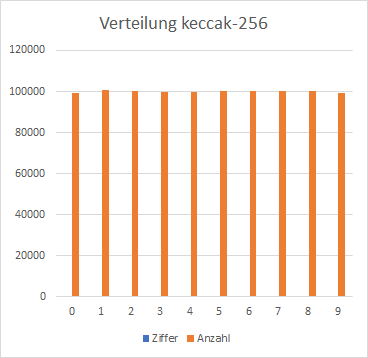
\includegraphics[width=\textwidth]{Figures/verteilung_keccak256}
\centering
\decoRule
\captionof{figure}{Verteilung der Keccak-256 Hashfunktion}
\label{fig:verteilung_keccak256}
\end{minipage}

\subsection{Sicherheit von Smart Contracts}
Bei Smart Contracts handelt es sich um öffentliche, für jeden ausführbare und unveränderliche Software. Beinhaltet diese einen Software-Fehler, ist dieser ausnutzbar und kann nicht behoben werden. Smart Contracts verwalten in der Regel Geld oder Token, die einen finanziellen Wert repräsentieren. Bei der Entwicklung eines Smart Contracts ist somit oberste Vorsicht geboten. Das Beispiel des Smart Contracts \textit{theDAO}\footnote{The DAO ist ein, als Smart Contract realisierter, Kapitalfond, der es sich zur Aufgabe gemacht hat in Blockchain Technologie zu investieren. Im April 2016 haben über elftausend Investoren Kapital von mehr als 150 Millionen Dollar in den Fond eingezahlt. Als Gegenleistung haben die Investoren eine entsprechende Anzahl Token als eine Art Stimmrecht erhalten. Investitionsentscheidungen werden von den Investoren durch einen dezentral erarbeiteten Konsens mithilfe des Smart Contracts getroffen. Smart Contract Code: \url{https://etherscan.io/address/0xbb9bc244d798123fde783fcc1c72d3bb8c189413\#code}} zeigt zu welchen fatalen Folgen eine Sicherheitslücke führen kann. Durch das Ausnutzen eines nicht trivialen Fehlers im Smart Contract Code schaffte es ein Hacker 3,6 Millionen Ether an eine von ihm kontrollierte Adresse auszuzahlen. Eine genaue Beschreibung des Angriffes findet man unter \cite{eth_dao_hack}.\\\\
Bezüglich der Sicherheit des Contracts Codes aus Abschnitt \ref{eth_smart_contract} gibt es 2 Angriffsfaktoren, die berücksichtigt werden müssen. Der Code der \code{payout} Funktion befindet sich zur Wiederholung am Ende der Seite.


\subsubsection{Wahl der Zufallsquelle}
Als Zufallsquelle dürfen keine durch Miner oder andere Teilnehmer manipulierbare Werte genommen werden. Beispielsweise würde die Verwendung des Statements \code{bock.timestamp(payoutBlockNumber)} in Zeile 4 der \code{payout} Funktion zu einer wesentlich größeren Angriffsfläche führen. Miner können in einem gewissen Rahmen entscheiden welchen Wert sie in das Timestamp-Feld des Blockheaders schreiben und somit die Ausführung des Codes manipulieren.
%In Zeile 4 der \code{payout} Funktion muss zwingend der Blockhash als Quelle für den Zufall genommen werden.
\subsubsection{Rekursive Auszahlung}
Verwendet man das Statement \code{winnerAddress.call.value(amount)} statt\\ \code{winnerAddress.transfer(amount)} in Zeile 12 zur Auszahlung, kann ein Angreifer eine mehrfache Auszahlung veranlassen indem er die Adresse eines vorher präparierten Smart Contracts als Auszahlungsadresse angibt. Sobald ein Smart Contract Ether empfängt, ohne dass dabei explizit eine Funktion aufgerufen wird (beispielsweise durch \code{address.call.value(amount)}), wird die \code{default} Funktion des Contracts aufgerufen. Präpariert der Angreifer die \code{default} Funktion nun so, dass diese die \code{payout} Funktion des Glücksspiel Contracts aufruft, kann er dadurch eine erneute Abarbeitung der \code{payout} Funktion bewirken. Da die \code{payout} Funktion keinen Schutz gegen eine erneute Abarbeitung besitzt, wird der Topfbetrag ein weiteres Mal auf die Adresse des Gewinners überwiesen.\footnote{Dies funktioniert nur, falls der Glücksspiel Contract genügend Ether besitzt. Außerdem muss der Angreifer einen Abbruchmechanismus in seiner \code{default} Funktion vorsehen.} Als Schutzmaßnahme ist es ratsam das Statement \code{potClosed = false} aus Zeile 15 an den Anfang der Funktion (beispielsweise in Zeile 4) zu verschieben, um einen rekursiven Aufruf zu verhindern. 

Die Solidity Dokumentation enthält eine Reihe von Beispielen \cite{solidity_security}, die die Sicherheit von Smart Contracts betreffen. Entwickler sollten sich dieser bewusst sein, bevor sie einen Smart Contract veröffentlichen der Geld verwaltet.

\begin{lstlisting}[basicstyle=\small]
function payout() public{
    assert(potClosed);
    assert(block.number>payoutBlockNumber);
    payoutBlockHash = block.blockhash(payoutBlockNumber); 
    if(payoutBlockHash == 0){
        nbrOfMissedPayouts++;
    }else{
        winner = uint256(payoutBlockHash) % NBR_OF_SLOTS;
        address winnerAddress = payoutAddresses[winner];
        uint amount= EXPECTED_POT_AMOUNT*NBR_OF_SLOTS;
        amount += EXPECTED_POT_AMOUNT*NBR_OF_SLOTS*nbrOfMissedPayouts;
        winnerAddress.transfer(amount); // send pot amount to winner
        nbrOfMissedPayouts = 0;
    }
    potClosed = false;
    nbrOfParticipants=0;
}
\end{lstlisting}


